\chapter{Methodology}
\label{sec:methodology}

%%%%%%%%%%%%%%%%%%%%% Kurze Einführung %%%%%%%%%%%%%%%%%%%%%

In this section, the methodology of this work is described.
In \autoref{sec:usedModels} used and implemented models are explained.
\autoref{sec:usedDatasets} describes datasets, which are used to train and evaluate models and other algorithms.
The data augmentation of these datasets is depicted in \autoref{sec:dataaugmentation}.
\autoref{sec:lossFunction} deals with loss functions.
After that, setups for training and inference measurements are described in \autoref{sec:trainigsSetup} and \autoref{sec:measuringInference}.
Keep in mind that the main contributions of this work include three parts:
%1. an initial approach to combine object detection with semantic segmentation;
%2. TEP-Net \cite{tepNet2024} is the new baseline for further experiments to improve this model's accuracy and robustness;
%3. An RNN is integrated into the model to increase robustness further;

\begin{enumerate}
    \item An initial approach to combine object detection with semantic segmentation.
    \item TEP-Net \cite{tepNet2024} is the new baseline for further improvements in accuracy and robustness.
    \item An RNN is integrated aiming to eliminate the limitation of single-frame-based approaches.
\end{enumerate}

%%%%%%%%%%%%%%%%%%%%%%%%%% Models %%%%%%%%%%%%%%%%%%%%%%%%%%

\section{Models}

In this section all models are discussed which are used or created in this work.
This section is divided into three subsections.
Each of them corresponds to one of the main contributions of this work.
Therefore the first section gives a brief overview of used object detection models, the second one with the \ac{TEP}-Net \cite{tepNet2024} because it is used as a baseline.
Additionally, further improvements of this model are described in this section.
The last section describes all temporal models.

\subsection{Object Detection Models}

The state of the art in \autoref{sec:ObjectDetection} shows that one-stage detectors have the most promising characteristics to be successfully utilized in this work.
The most interesting ones are the models from the \ac{YOLO} series, especially the most recent ones because they focus on improved parameter usage.
This makes the models light weight and presents an advantage for this work, because operation on limited hardware is aimed for.
At the start of this work the most recent model from the \ac{YOLO} series is the \ac{YOLO}v9 \cite{YOLOv9}.
For object detection different models of the \ac{YOLO}v9 and the \ac{GELAN} series are available.
However, the \ac{YOLO}v9 models were not fully supported at that time.
Therefore the models used for experiments include the \ac{GELAN}-c and \ac{GELAN}-e.
These are obtained trough the GitHub repository \cite{YOLOv9GitHub} and used unchanged.
An additional model which is used for experiments is the \ac{YOLO}v7 \cite{yolov7} model, which is also utilized unchanged from the GitHub repository \cite{YOLOv7GitHub}.

\subsection{TEP-Net Model}
\label{subsec:baselineModel}

In the literature rails are often detected without distinction between all rails visible in an image and the rail the train continues.
\cite{tepNet2024} therefore proposes a regression-based approach, which restricts the model to predict a single track.
The idea comes from various lane detection methods in autonomous driving applications for road cars and is fitted to the rail domain.
Since, this method fits well to the goal of this work, it is used as a baseline for further experiments.

Although rails can be represented by second or third-degree polynomials most of the time \cite{PolyLaneNetRoad2021}, they may also take more complex geometric shapes.
Hence, limiting the output to presumed forms is discouraged.
Therefore, the method used in \cite{tepNet2024} employs spline interpolation to describe such complex structures.

\begin{figure}[H]
    \centering
    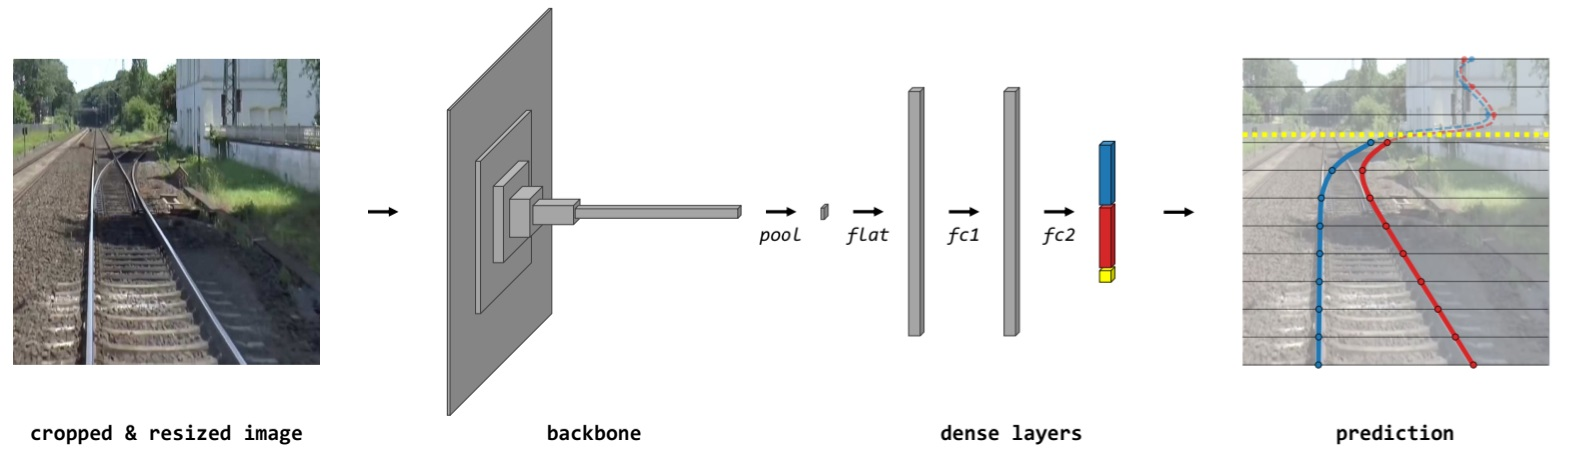
\includegraphics[width=\linewidth]{PICs/Baselinepaper/TEP-Net_model.jpg}
    \caption{\ac{TEP}-Net model architecture\cite{tepNet2024}. The input of the model is a cropped and resized image and the output of the model are the $x$-values for the left and right rail on each anchor line plus an additional value for the $y$-limit.}
    \label{fig:TEP-Net_model}
\end{figure}

As shown in the prediction of \autoref{fig:TEP-Net_model}, a set of horizontal lines are overlayed in the cropped image.
The number of $y$-lines or "anchors" is determined by a hyperparameter.
They are uniformly distributed along the $y$-axis. For each line, two $x$-values are predicted.
One for the left rail and one for the right rail.
The prediction image of \autoref{fig:TEP-Net_model} and the second and fourth images in the bottom row of \autoref{fig:tepNet_dataaugmentation} show that rails do not necessarily cross with anchor lines at the top of image crops.
Therefore, an additional $y$-limit is predicted, which gives information up to which anchor the rail should be detected.
Anchors and their $x$-values above this horizon line do not hold valuable information and are ignored.

For this novel regression task, a new model architecture is created.
For this model widely used backbone architectures like ResNet and EfficientNet are chosen.
The input of the backbones is an image crop with the size of $3 \times 512 \times 512$ which represents a rough average of crops obtained by data augmentation strategies.
These backbones extract relevant features from these crops reducing the spatial dimensions and increasing channel size to a high number.
After that, the feature map's number of channels is reduced to a predefined size with a 1x1 Conv2d layer \cite{pytorch_conv2d_docu} and flattened to a vector.
This feature vector serves as the input for the prediction head, which consists of two fully connected layers \cite{pytorch_linearLayer_docu} in series.
The size of the linear layers is set with a hyperparameter.
In the last layer, a reduction leads to the resulting prediction vector with the dimension $2 \times H + 1$.
This vector includes the entire information of one prediction.
$H$ is the number of anchors.
The first set of values with size $H$ is for the left rail, another $H$ set for the right rail and the $+ 1$ is for the last values being the horizon line.

This architecture's policy for value ranges does not restrict the $x$-values in any way.
This way predictions can be outside of a crop and the model can learn that sometimes the rails extend out of the viewed field.
The $y$-limit on the other hand is constrained to a range between 0 and 1 with a Sigmoid function.

The introduced model architecture can be classified as an end-to-end framework.
This means the model can be trained and used for inference without any steps in between.
It takes in raw data and results in a complete prediction.


\subsection{Improvements to the TEP-Net Model}
\label{subsec:improvemensts2BaselineModel}

One of the main contributions of this work is to improve the chosen baseline model from \cite{tepNet2024}.
These improvements can be roughly divided into three parts.
First, the backbones are exchanged with other architectures.
Secondly, after the backbones, a true pooling layer is integrated.
Thirdly, experiments with different prediction heads are conducted.
The following sections describe the structure of these architecture changes in detail.

\subsubsection{Backbones}

Backbones are used for extracting features from images.
These are parts of \ac{CNN}s that input and output tensors.
Common \ac{CNN} architectures usually work with 4D tensors with $B \times C \times H \times W$ as shown in \autoref{fig:backboneLogic}.
$B$ is the batch size, $C$ is the channel size, $H$ and $W$ are the height and width of the input image.
The backbone transforms this high-level feature map into a low-level one with different operations, resulting in a tensor with a high number of channels $C$ and low numbers in resolution $H$ and $W$.
The batch size $B$ tells how many images the \ac{CNN} processes simultaneously and stays the same.
These characteristics apply to all four chosen backbones.
As described in the state of the art in \autoref{sec:networkArchitectures}, the most interesting models are ResNet \cite{ResNet}, EfficientNet \cite{EfficientNet}, DenseNet \cite{DenseNets}, and MobileNetV3 \cite{MobileNetV3}.
ResNet and EfficientNet are already implemented in \cite{tepNet2024}.
DenseNet and MobileNet are additionally integrated in this work.
\autoref{tab:backboneVersions} gives an overview of all different versions which are implemented in this work.

\begin{table}[H]
    \centering
    \begin{tabular}{|l|l|}
    %\begin{tabular}{| p{0.3\linewidth} | p{0.6\linewidth} |}
        \hline
        ResNet & 18, 34, 50\\
        \hline
        MobileNetV3 & small, large\\
        \hline
        DenseNet & 121, 161, 169, 201\\
        \hline
        EfficientNet & B0, B1, B2, B3\\
        \hline
    \end{tabular}
    \caption{Versions of backbones utilized in this work}
    \label{tab:backboneVersions}
\end{table}

\begin{figure}[H]
    \centering
    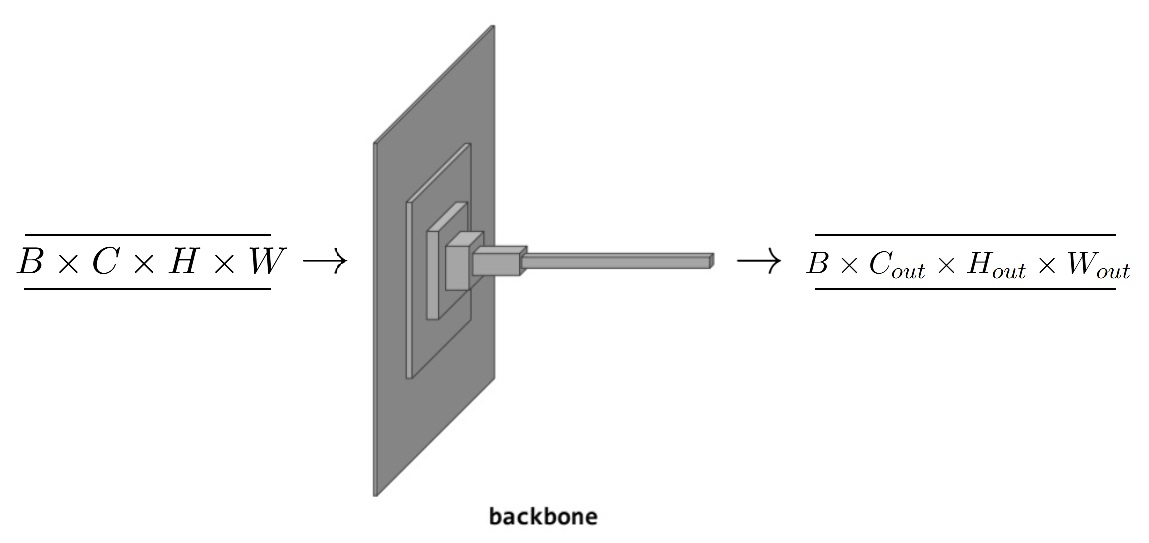
\includegraphics[width=0.6\linewidth]{PICs/improvedModel/backbone_logic.jpg}
    \caption{Backbone logic (backbone graphic taken from\cite{tepNet2024}).}
    \label{fig:backboneLogic}
\end{figure}

When exchanging backbone architectures it is important, that the dimensions of input and output tensors are the same for every backbone otherwise the next layers would get different input dimensions than they are designed for.
Standardizing the input tensor is done by resizing an image to $512 \times 512$ after augmentation.
While $B$ is set by a hyperparameter, $C = 3$ because images are in the 3-channel \ac{RGB} format.
For the output dimensions, the backbone architectures and their operations must be analyzed.
When inspecting all four backbones in more detail it becomes clear that they all share the following characteristics:

\begin{itemize}
    \item The input resolution in all papers is $224 \times 224$.
    \item At the end, there is either a pooling layer, a $1 \times 1$ convolutional layer, or both in combination with fully connected layers forming a prediction head for classification tasks.
    \item Before the prediction head, the spatial resolution of feature maps is $7 \times 7$.
\end{itemize}

With this information, the last layers of each backbone can be discarded, so all backbones output tensors with the same $H$ and $W$.
In all four papers, the architecture transforms tensors with a resolution of $224 \times 224$ to a tensor with $7 \times 7$ before the prediction heads.
This means they all have the same reduction factor of 32.
Since the input resolution of $512 \times 512$ is used in this work resulting feature maps have a resolution of $16 \times 16$ after backbones.
The exact dimensions of all tensors are shown in \autoref{tab:backboneDimensions}.

\begin{table}[H]
\centering
\begin{tabular}{|r|p{0.2\linewidth}|r@{ }r@{,  }r@{,  }r@{,  }r@{ }l|}\hline
%\begin{tabular}{| p{0.3\linewidth} | p{0.3\linewidth} | p{0.3\linewidth} |}\hline
\multicolumn{1}{|l|}{\textbf{Backbone}}       & \textbf{Input dimensions} & \multicolumn{6}{|l|}{\textbf{Output dimensions}}\\\hline
ResNet                  & \multirow{4}{=}{\centering [ 8, 3, 512, 512 ]}  & [ & 8 &  512 & 16 & 16 &]\\\cline{1-1} \cline{3-8}
MobileNetV3             &                                               & [ & 8 &   96 & 16 & 16 &]\\\cline{1-1} \cline{3-8}
DenseNet                &                                               & [ & 8 & 1024 & 16 & 16 &]\\\cline{1-1} \cline{3-8}
EfficientNet            &                                               & [ & 8 &  384 & 16 & 16 &]\\\hline
\end{tabular}
\caption{Versions of backbones utilized in this work}
\label{tab:backboneDimensions}
\end{table}

\subsubsection{Pooling Layer}

blindtext

\subsubsection{prediction Heads}

\begin{figure}[H]
    \centering
    \begin{subfigure}[t]{0.2\textwidth}
        \centering
        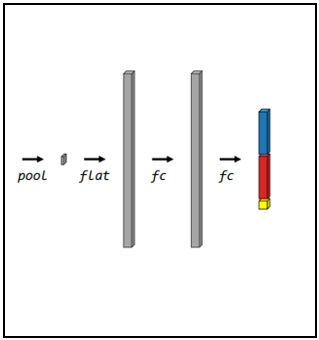
\includegraphics[height=3.35cm, keepaspectratio]{PICs/improvedModel/originalHead.jpg}
        \caption{Original Head \cite{tepNet2024}}
    \end{subfigure}
    \begin{subfigure}[t]{0.3\textwidth}
        \centering
        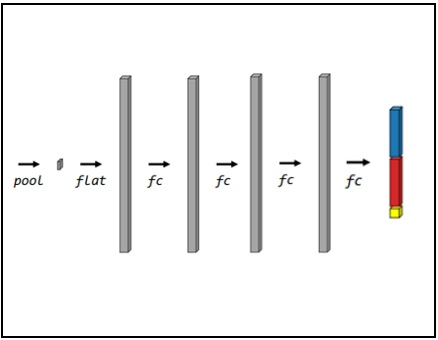
\includegraphics[height=3.35cm, keepaspectratio]{PICs/improvedModel/depthHead.jpg}
        \caption{Depth Head}
    \end{subfigure}
    \begin{subfigure}[t]{0.25\textwidth}
        \centering
        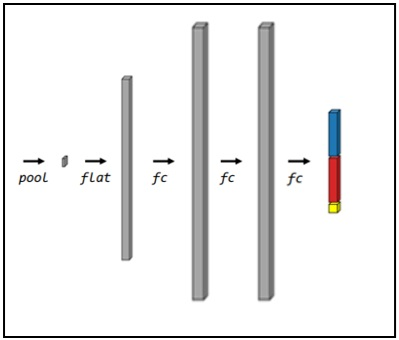
\includegraphics[height=3.35cm, keepaspectratio]{PICs/improvedModel/widthHead.jpg}
        \caption{Width Head}
    \end{subfigure}
    \begin{subfigure}[t]{0.3\textwidth}
        \centering
        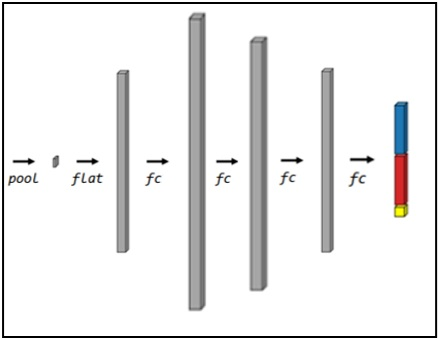
\includegraphics[height=3.35cm, keepaspectratio]{PICs/improvedModel/trapezHead.jpg}
        \caption{Trapez Head}
    \end{subfigure}
    \caption{Different architectures for prediction heads.}
\end{figure}

blindtext



%%%%%%%%%%%%%%%%%%%%%%%%%% Datahandling %%%%%%%%%%%%%%%%%%%%%%%%%%

\section{Data handling and Training process}
\label{sec:datahandling}

\begin{figure}[H]
    \centering
    \begin{tikzpicture}[every node/.style={font=\tiny}]
        \tikzstyle{block} = [rectangle, rounded corners, draw=black, minimum width=2.5cm, minimum height=1.5cm, align=center, anchor=center]
    
        \newcommand{\emphasize}[1]{\scriptsize{\textbf{#1}}}
        \def\vsep{.6cm}
        \def\hsep{2cm}
    
        % linke Abfolge
        \node (image) at (0,0) [block] {\emphasize{Image} (RGB)};
        \node (Dataset)     [block, below=\vsep of image, align=center]     {\emphasize{Dataset}\\Data Augmentation\\out: [C, H, W]};
        \node (Dataloader)  [block, below=\vsep of Dataset, align=center]   {\emphasize{Dataloader}\\divides into batches\\out: [B, C, H, W]};
        \node (Model)       [block, below=\vsep of Dataloader, align=center]{\emphasize{Model}};
    
        % rechte Abfolge 
        \node (Video)       [block, right=\hsep of image, align=center]         {\emphasize{Video}};
        \node (Dataset2)    [block, below=\vsep of Video, align=center]         {\emphasize{Dataset}\\Data Augmentation\\out: [S, C, H, W]};
        \node (Dataload2)   [block, below=\vsep of Dataset2, align=center]      {\emphasize{Dataloader}\\divides into batches\\out: [B, S, C, H, W]};
        \node (TempModel)   [block, below=\vsep of Dataload2, align=center]     {\emphasize{Temporal Model}};
        \node (Sampler)     [block, right=.5*\hsep of Dataload2, align=center]  {\emphasize{Sampler}\\indexing for\\sequences};
    
        % Überschriften
        \node   [align=center, above=.2cm of image] {\emphasize{Single frame training Process}};
        \node   [align=center, above=.2cm of Video] {\emphasize{Temporal training Process}};
    
        \draw[-Stealth, thick] (image)       -- (Dataset);
        \draw[-Stealth, thick] (Dataset)     -- (Dataloader);
        \draw[-Stealth, thick] (Dataloader)  -- (Model);
    
        \draw[-Stealth, thick] (Video)            -- (Dataset2);
        \draw[-Stealth, thick] (Dataset2)         -- (Dataload2);
        \draw[-Stealth, thick] (Dataload2)        -- (TempModel);
        \draw[Stealth-Stealth, thick] (Dataload2) -- (Sampler);
        
    
    \end{tikzpicture}
    \caption{Comparison between data handling processes for single-frame training and the proposed temporal training.}
    \label{fig:dataHandlingProcess}
\end{figure}

The Dataset class reads images according to an index, performs online data augmentation, and outputs a tensor.
In the Dataset class also the targets are formed out of the augmented annotations.
First Polylines are transformed into a mask, then the data augmentation from \autoref{sec:dataaugmentation} is applied.
In the last step, this augmented mask is used to generate regression or classification targets.
For semantic segmentation, the mask can be utilized directly.
The Dataloader iterates through the dataset step by step and calls the dataset class using indices.
It can either move step by step or rely on a sampler to dictate the stepping pattern.
In temporal training, a sampler is essential for managing sequences, avoiding out-of-bound errors, and preventing scene intermixing.
A sliding window approach is implemented, shown in \autoref{fig:slidingWindow}.
A window of a predefined number of images serves as input for the model.
This number (usually 10) is smaller than the sequence length of 76.
Then the data loader steps through the sequence.
At the end of a sequence, the sampler forces the Dataloader to jump to the next sequence instead of mixing them.
Furthermore, the Datalaoder creates batches and therefore adds the dimension $B$ to the tensor.

\begin{figure}[H]
    \centering
    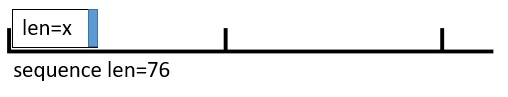
\includegraphics[width=0.5\linewidth]{PICs/usedDatasets/slidingWindow.jpg}
    \caption{Sampler is responsible for the sliding window approach in temporal training: bottom line represents the sequence with a length of 76 frames; the box is the window of frames used as the input for the model with x being the length of this window (with $x \leq 76$); the blue part of the sliding window represents the output frame because this temporal method deals with a sequence-to-one problematic.}
    \label{fig:slidingWindow}
\end{figure}

\noindent The training consists of a pre-defined number of epochs, which presents one training cycle.
In each epoch, the Dataloader is used to feed the model one batch.
Then the model predicts, calculates the loss according to this prediction, and performs the back propagation to optimize the model.
In the same cycle, the validation is done, in which the Dataloader feeds the model samples of the validation set.
Here only the prediction is done and the loss is calculated.
Two additional steps are done in an epoch after training and validating.
On the one hand, the OneCycleLR scheduler \cite{pytorch_oneCycleLR_docu} is used to update the learning rate.
On the other hand, a model is saved as the best one as soon as it reaches a new minimum in the validation loss.
This way the model with the lowest loss is obtained.


%%%%%%%%%%%%%%%%%%%%%%%%% Datasets %%%%%%%%%%%%%%%%%%%%%%%%%

% RailSem19 for Yolos + used subsets [1/2 bis 1 Seite]
% TEP-annotations [1/2 Seite bzw. ein kurzer Absatz]
% Switch evaluation dataset (all images with switches from val and test dataset) [1/2 Seite bzw. ein kurzer Absatz]
% auto labler + temporal dataset + dass ich CVAT versendet habe[1 bis 2 Seiten]

\section{Datasets}

\begin{itemize}
    \item RailSem19 for Yolos + used subsets [1/2 bis 1 Seite] fertig
    \item TEP-annotations [1/2 Seite bzw. ein kurzer Absatz] fertig
    \item Switch evaluation dataset (all images with switches from val and test dataset) [1/2 Seite bzw. ein kurzer Absatz]
    \item auto labler + temporal dataset + dass ich CVAT versendet habe[1 bis 2 Seiten]
\end{itemize}

\subsection{RailSem19 and subsets for training object detection models}

The first approach to creating a Rail Track Prediction system includes combining an object detection model with a semantic segmentation model.
Since RailSem19 supports both of these methods this dataset is chosen for training.
Furthermore, state-of-the-art research in \autoref{sec:datasets} shows that this dataset is the only one that not only includes switch annotations but also labels for switch states: $switch\_left$, $switch\_right$.
Since not all states are identifiable even though a switch is visible there also is the $switch\_unknwon$ label.

In this work, the bounding boxes are utilized to train the \ac{YOLO} object detection models.
Experiments have been conducted with three versions of this dataset.
An overview of these subsets is shown in \autoref{tab:usedSubsetsforYOLOs}.
The first set is the whole dataset, which includes 8500 images with all different bounding box labels.
The second subset only considers images with switch labels including the $switch\_unknown$ label.
For this subset, 2764 images remain. The third subset only considers the switch labels in which the state is identifiable.
This is because when focusing on the direction the train takes, the $switch\_unknown$ label does not hold any valuable information.
To prevent confusion, all images containing $switch\_unknown$ annotations are intentionally excluded, resulting in a final set of 1,240 images.

\begin{table}[H]
    \centering
    \begin{tabular}{|l|l|l|}
    %\begin{tabular}{| p{0.3\linewidth} | p{0.6\linewidth} |}
        \hline
        \textbf{RailSem19} & \textbf{RailSem19\_onlySwitches} & \textbf{RailSem19\_onlySwitchesLeftRight}\\
        \hline
        8500 images & 2764 images & 1240 images\\
        \hline
        all bounding box labels & $switch\_left$ & $switch\_left$\\
        \hline
        & $switch\_right$ & $switch\_right$\\
        \hline
        & $switch\_unknown$ & images with $switch\_unknown$ excluded\\
        \hline
    \end{tabular}
    \caption{Used dataset subsets of RailSem19 for training \ac{YOLO} object detection models}
    \label{tab:usedSubsetsforYOLOs}
\end{table}

Since the experiments of training object detection models showed unsatisfactory results also described in <section>, this methodology was deemed ineffective.
This leads to the pursuit of a different solution and experiments with semantic segmentation models are therefore not accomplished.
Consequently the corresponding dense labels of the RailSem19 dataset are not utilized.

\clearpage
\subsection{TEP annotations}

For training single-frame-based models \cite{tepNet2024} published its annotations for the images of RailSem19.
These annotations consist of polylines for the left and the right rail of the train.
Only the two rails are included in the labels which the train drives on.
This is also the case when switches are present.
Additionally, some images are excluded from this dataset when the train's track is not identifiable.
For labeling this dataset the online tool CVAT \cite{cvat} is used.
These annotations can then be transformed with pre processing step to support other models like semantic segmentation. 
This dataset is described in more detail in \autoref{subsubsec:TEP-Net_dataset}.

\subsection{Switch evaluation dataset}

blindtext

\subsection{Temporal Dataset}

blindtext


%%%%%%%%%%%%%%%%%%%% Data augmentation %%%%%%%%%%%%%%%%%%%%%

%grobe Einteilung:
% - Data augmentation for Training
% - Data augmentation for Temporal Training
% - Cropping in inference
% - improved auto crop 

\section{Data augmentation}
\label{sec:dataaugmentation}

In this section a thorough explanation of the data augmentation of \cite{tepNet2024} is given, for training and the cropping augmentation for inference.
Additionally, all data augmentation strategies that are used in this work are described.
%This includes a brief description of Yolos data augmentation.
This includes the methods adapted for training temporal models and an improved "Autocropper" technique for inference.

\subsection{Data augmentation for Training single-frame-based models}

\cite{tepNet2024} utilizes three data augmentation techniques in the training process.
The first two are commonly used in \ac{CV} tasks, including random horizontal flips and traditional image adjustments like brightness, contrast, saturation, and hue variations.
For this, the standard ColorJitter \cite{pytorch_colorJitter_docu} method from PyTorch is used.
The third augmentation is the cropping mechanism, which reduces the image to the most relevant part.
Randomness is also introduced to enhance generalization.

\autoref{fig:tepNet_dataaugmentation} visualizes the cropping algorithm steps schematically.
The \ac{GT} is in the form of polylines and are represented by the two green lines.
Then the yellow rectangle is computed, being the smallest possible rectangle around the \ac{GT}.
In the next step, the start pixels of the rails \ac{GT} are centered by expanding the yellow borders in one direction resulting in the orange box.
All start pixels of rails are in the lowest row of an image.
After that margins are added shown by the red rectangle.
These margins are predefined with hyperparameters.
After calculating the borders of the outermost box, variability is added to enhance generalization and prevent biases.
The left, right, and top borders are moved by a distance calculated with a predefined normal distribution.
This introduced variability follows the policy, which ensures that the starting pixels of the rails at the bottom stay in the cropped image.
\autoref{fig:tepNet_dataaugmentation} illustrates four augmented variations of the top image in the bottom row.

\begin{figure}[H]
    \centering
    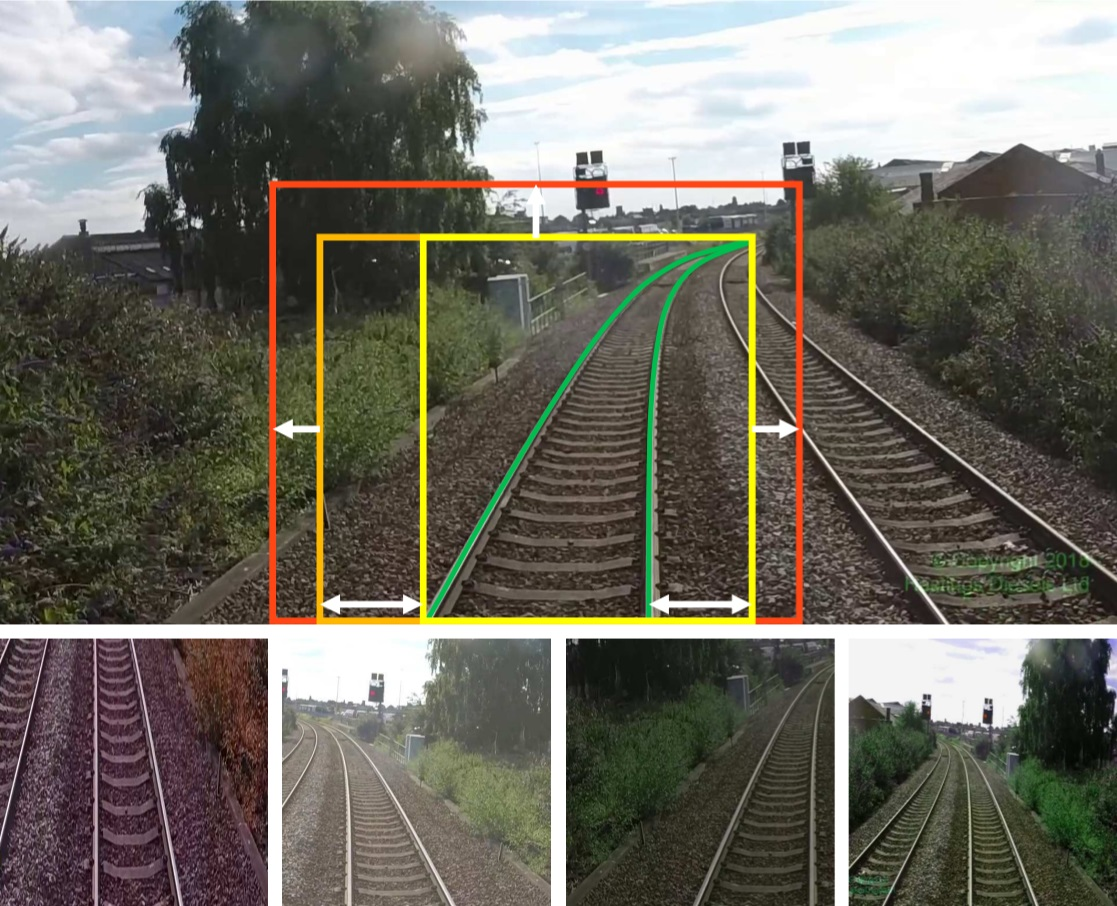
\includegraphics[width=0.6\linewidth]{PICs/Baselinepaper/data_augmenation.jpg}
    \caption{Data augmentation of \ac{TEP}-Net \cite{tepNet2024}, including the image horizontal flips, the color variations and the cropping mechanism.}
    \label{fig:tepNet_dataaugmentation}
\end{figure}

\subsection{Data augmentation for Training temporal models}
\label{sec:dataAugmentationTemporal}

For training temporal models the same three data augmentation strategies as the ones from training single-frame-based models are utilized for enhanced generalization.
These again include horizontal flips, color variations, and a similar cropping mechanism.
However, when training a model with sequences of images, the same augmentation must be used on all images of this sequence.
For the first two augmentation techniques, random values are obtained and saved in variables.
Then these random factors are applied to each image in the sequence.
For the horizontal flip, a threshold at $0.5$ and a random value between $0$ and $1$ define if a sequence is flipped or not.
To achieve the same effect as the ColorJitter \cite{pytorch_colorJitter_docu} function from the single-frame training, four uniform distributions are implemented outputting random values for brightness, contrast, saturation, and hue.
These are then the parameters for the functions: \texttt{adjust\_brightness} \cite{pytorch_adjust_brightness_docu}, \texttt{adjust\_contrast} \cite{pytorch_adjust_contrast_docu}, \texttt{adjust\_saturation} \cite{pytorch_adjust_saturation_docu}, and \texttt{adjust\_hue} \cite{pytorch_adjust_hue_docu}.

The cropping mechanism needs more consideration.
First, the same method as the one from single-frame training is applied to the first image of a sequence to obtain the red borders shown in \autoref{fig:tepNet_dataaugmentation}.
To still guarantee randomness to minimize the risk of unwanted biases, the location of the left, right, and top borders are moved according to a normal distribution.
To assure consistency along a sequence, the distances between the red borders and the random borders are calculated.
From this point on the red borders are calculated in every image as before and these distances are used to incorporate random factors, instead of new random values for every image.
The whole algorithm still follows a policy that the starting pixels of the rails stay in the image crop.
\autoref{fig:temporalDataAugmentation} visualizes an example sequence with raw images in the top row and augmented crops in the bottom row.
The first, middle, and last images of a sequence with 10 images are shown.
The train's progress is most clearly visible through the pole of the overhead line. 


\begin{figure}[H]
    \centering
    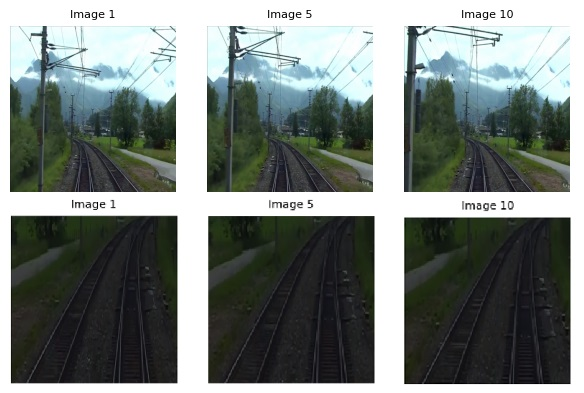
\includegraphics[width=0.7\linewidth]{PICs//dataAugmentation/temporal_data_augmentation.jpg}
    \caption{Data augmentation for temporal data processing, including the 1\textsuperscript{st}, 5\textsuperscript{th} and 10\textsuperscript{th} image of a sequence. First row resized raw images. Second row augmented images with the same three augmentation techniques for the whole sequence.}
    \label{fig:temporalDataAugmentation}
\end{figure}

\subsection{Cropping in inference with TEP's Autocrop}

In \cite{tepNet2024} only cropped images are used for training models to only consider the most relevant \ac{ROI} in images.
For training and validating the model on the dataset, the \ac{GT} allows the computation of crop coordinates (left, top, right).
However, \ac{GT} data is unavailable in practical applications like video inference.
As a result, the crop coordinates must be, either predefined by a user or computed on the fly.

In a real-world application the ROI in the images changes, even when the camera is mounted in a fixed position.
Because of these perspective shifts when the train drives right or left turns, it easily can become unsustainable to have predetermined crop coordinates.
\autoref{fig:perspective_shifts} visualizes these perspective shifts.
The tighter the curve, the worse the shift.
The approach of \cite{tepNet2024} to solve this particular problem is the so-called "Autocrop".
This developed technique starts with the whole image, so the initial crop coordinates are the image borders.
After the initialization, the three coordinates (left, top, right) are updated according to the prediction of every new frame.
In more detail, new coordinates are calculated with a running average of the smallest rectangle around the prediction plus the predefined margins from the training.
Furthermore, the global averages of crop coordinates are taken in consideration.
This allows the crop coordinates to converge to these global averages and prevent collapse scenarios, in which the crop becomes to small.


\begin{figure}[H]
    \centering
    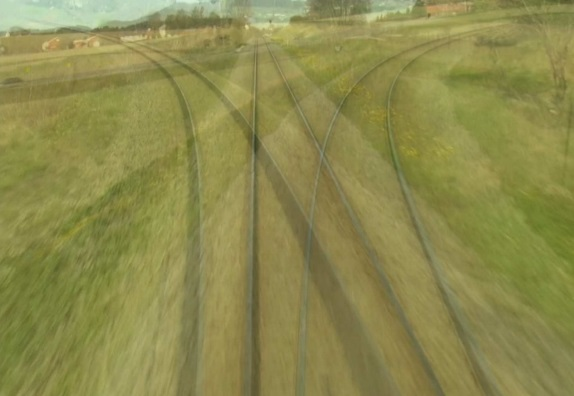
\includegraphics[width=0.6\linewidth]{PICs/Baselinepaper/perspective_shifts.jpg}
    \caption{Example of perspective shifts with three different scenarios: left curve, right curve and straight rail \cite{tepNet2024}.}
    \label{fig:perspective_shifts}
\end{figure}

\subsection{Improved Autocrop for inference}
\label{sec:imporvedAutocrop}

\cite{tepNet2024} incorporates a \ac{RA} \autoref{func:runningAverage} with rule-based policies to prevent collapse to the inside and consider image borders when adding a margin. After that, the newly calculated and checked average is weighted and added to form the new crop coordinates, like in \autoref{func:weightingAverage}. In these formulas $AVG$ is the average, $x$ is the crop coordinates and $pred$ is the values obtained from the prediction. In \autoref{func:weightingAverage} the same annotations are used with $c$ being the coefficient, which is 0.1. All notations but $c$ include all three crop coordinates: left, top right.

\begin{align}
    AVG_t = \frac{AVG_{t-1} \cdot (t-1) + pred_t}{t}
    \label{func:runningAverage}
\end{align}

\begin{align}
    x_{t} = x_{t-1} * (1 - c) + AVG_{t} * c
    \label{func:weightingAverage}
\end{align}

However, observations in the inference of videos demonstrate that the introduced autocrop mechanism is not optimal. The behavior shows that the \ac{RA} reacts slowly to the inside and the outside. This is especially problematic when the crop should quickly expand in one direction. Additionally, the borders of the crop converge to an overall average, presenting the same issues as when simply pre-defining a crop. Those behaviors can push the prediction outside the rails. In more detail when the rails move to the left or right in the image due to a perspective shift when the train takes a curve and the Autocroper does not react quickly enough, the rails are subsequently positioned outside the crop area. An additional issue presents the lack of an recovery option when the image crop is completely incorrect.

\begin{align}
    x_t =  x_{t-1} * (1 - c) + pred_t * c
    \label{func:EMA}
\end{align}

Therefore a new algorithm is implemented for this work to present a more robust solution.
The desired behavior should be one that is more responsive to the outside to react to rapid changes in perspective.
Simultaneously, the crop should converge gradually to the inside to prevent any fast movements of crop coordinates, which possibly lead to collapse events.

To realize such an algorithm an \ac{EMA} is utilized shown in \autoref{func:EMA}, in which only the old crop coordinates and the values from the prediction are weighted and added.
$c$ is the coefficient which is set to 0.01 presenting slow movements to the inside.
Additionally, with the same collapse prevention technique as before the crop cannot be smaller than the smallest rectangle of the prediction (yellow box in \autoref{fig:tepNet_dataaugmentation}).
However, by directly calculating the crop coordinates without any averages in between like \autoref{func:runningAverage}, this leads to a different behavior.
The collapse prevention rule now overwrites the coordinates when the prediction expands, resulting in a rapid widening of the crop.

Furthermore, the crop is bound to stay within image borders.
Further adaptations to enhance robustness are done by increasing the margins, which are added to the prediction rectangle (yellow box in \autoref{fig:tepNet_dataaugmentation}) to give the model more leeway.

Additionally, a reset rule is implemented in which the crop coordinates are overwritten with predefined values.
The behavior is observed that when models become uncertain, the horizon line converges to the bottom of the image.
This behavior is used and the crop resets when the predicted horizon line is below 40\% of the crop height.
Experiments show that the following reset values are the most advantageous: left = 1/3 of image width, top = 1/2 of image height, right = 2/3 of image width.



%%%%%%%%%%%%%%%%%%%%%% Loss function %%%%%%%%%%%%%%%%%%%%%%%

\section{Loss function}
\label{sec:lossFunction}

One of the main contributions of \cite{tepNet2024} is the loss function, which is tailored to the particular problem formulation of the regression-based approach.
Since, this loss function demonstrates to be functional, it is adopted unchanged in this work.
This loss function \autoref{func:combinedLoss} \cite{tepNet2024} consists of two sub-functions, where the outputs are added together, with the $y$-limit loss weighted by a multiplication factor of $\lambda=0.5$ before summing.

\begin{align}
    L = L_{traj} + \lambda \times L_{ylim}
    \label{func:combinedLoss}
\end{align}

The two sub-functions are the trajectory loss $L_{traj}$ and $y$-limit loss $L_{ylim}$.
For the following functions, $\hat{\mathbf{X}}$ and $\mathbf{X}$ represent the predicted and \ac{GT} $x$-values.
These include the points for the left and right rails.
For the $y$-limit, the predicted and \ac{GT} values are $\hat{y}_{lim}$ and $y_{lim}$.

\vspace{1cm}

\noindent \textbf{Trajectory Loss} $L_{traj}$ determines the error between the predicted and actual $x$-values.
To calculate this error, the sum of smoothL1 is used as shown in the numerator \autoref{func:trajectoryLoss}.
This is done with a $\beta_{1} = 0.005$. As shown in figure \autoref{fig:smoothL1}, this function allows a linearly proportional relationship between loss and error.
Additionally, for noise in the data, it includes a smooth transition at zero.

One issue of the front view perspective is the so-called linear perspective effect.
This effect occurs when rails continue into the distance.
The same pixel error represents a small distance when near the camera's capturing point and a larger distance when far away.
This ratio grows linearly the greater the distance to the camera.
To counteract this effect, the results of the $L_{rails}(\hat{\mathbf{X}}_{i},\mathbf{X}_{i})$ are multiplied by the $w_{i}$ factor, which is inversely proportional to the width of the rail.
To prevent distortion of the results due to unreasonable weighting $W_{max}$ is used.
This value is the %95^{\text{th}}
percentile of all $w_{i}$ values from the training set.
This value is around 20 when data augmentation is used.

The $m_{i}$ factor is used to zero out and ignore all values above the $y$-limit.
Furthermore, it is ensured that the averaging of the loss is conducted exclusively over the relevant segment of the track.
This is done by summing all $m_{i}$ values in the denominator of \autoref{func:trajectoryLoss}.

%trajectory loss function
\begin{align}
    L_{traj} = \frac{\sum_{i=1}^H m_{i} \times w_{i} \times L_{rails}(\hat{\mathbf{X}}_{i},\mathbf{X}_{i})}
    {\sum_{i=1}^H m_{i}}
    \label{func:trajectoryLoss}
\end{align}

% smooth L1 error function
\begin{align}
    L_{rails} = \sum_{\substack{r \in \{left, right\}}} SmoothL1(\hat{\mathbf{X}}_{i,r} - \mathbf{X}_{i,r}, \beta_1)
    \label{func:smoothL1_error}
\end{align}

% Smooth L1
\begin{align}
    SmoothL1(x, \beta) = 
    \begin{cases}
        0.5 x^2 / \beta, & \text{if } |x| < \beta \\
        |x| - 0.5 * \beta, & \text{otherwise}
    \end{cases}
    \label{func:smoothL1}
\end{align}

% perspective weight function
\begin{align}
    w_{i} = \min \left( \frac{1}{\mathbf{X}_{i,right} - \mathbf{X}_{i,left}} , W_{max} \right)
    \label{func:perspective_weight}
\end{align}

% making factor
\begin{align}
    m_i = 
    \begin{cases} 
        1 & \text{if } i \leq y_{lim} \times H \\
        0 & \text{otherwise}
    \end{cases}
    \label{func:maskingFactor}
\end{align}

\vspace{1cm}

\noindent \textbf{Y-Limit Loss} $L_{ylim}$ is responsible for calculating the error of the horizon line.
For this sub-function also the $SmoothL1$ loss is taken with a $beta_{2} = 0.015$.
The value of $\beta_{2}$ is chosen to be higher, because of greater inaccuracy of annotations.
Due to images of the dataset stemming from low-resolution YouTube videos, it becomes difficult to accurately label the horizon line, especially when the end of the rail track is located at a significant distance.

\begin{align}
    L_{ylim} = SmoothL1(\hat{y_{lim}} - y_{lim}, \beta_{2})
    \label{func:ylimLoss}
\end{align}

\autoref{fig:smoothL1} shows a plot of the \autoref{func:smoothL1} being the $SmoothL1$ Loss function which is widely used in the literature.

\vspace{1cm}

\begin{figure}[H]
    \centering
    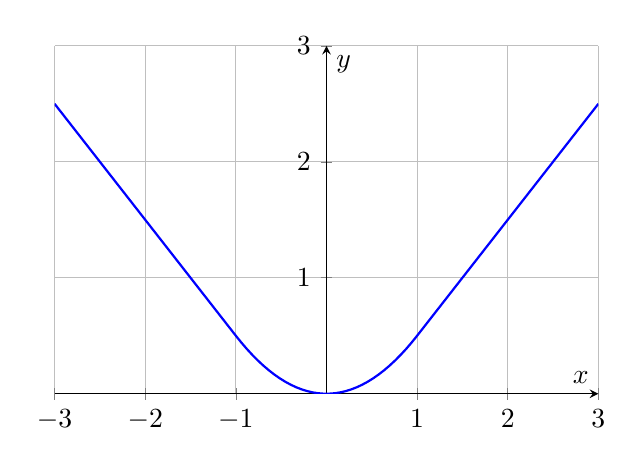
\begin{tikzpicture}
        \begin{axis}[
            title={},
            xlabel={$x$},
            ylabel={$y$},
            grid=major,
            domain=-3:3, % Bereich der x-Achse
            samples=100, % Anzahl der Punkte
            axis lines=middle, % Achsen durch die Mitte
            %xmin=-3, xmax=3, % Zoom Bereich auf der x-Achse
            width=0.7\textwidth, % Breitere Grafik
            height=6cm, % Schmalere Höhe der Grafik
            ymin=0.0, ymax=3, % Zoom Bereich auf der y-Achse
        ]
            % SmoothL1-Funktion
            \addplot[
                blue, 
                thick
            %]{abs(x) < 0.005 ? 0.5 * (x^2) / 0.005 : abs(x) - 0.5 * 0.005};
            ]{(abs(x) < 1) * (0.5 * x^2) + (abs(x) >= 1) * (abs(x) - 0.5)};
        \end{axis}
    \end{tikzpicture}
    \caption{$SmoothL1$ Loss Function}
    \label{fig:smoothL1}
\end{figure}


%%%%%%%%%%%%%%% Setup used for Training CNNs %%%%%%%%%%%%%%%

\clearpage
\section{Setup used for Training CNNs}
\label{sec:trainigsSetup}

% Hardware (GPU, CPU, CUDA)
For training \ac{CNN}s, a powerful hardware setup is necessary.
In this work, one main setup is used to train all models.
This work is based on a project proposed and supported by the \ac{ICT} at the \ac{TU}, which also provides the necessary resources.
The department has a server with two NVIDIA Tesla V100S-PCIE-32GB \ac{GPU}s \cite{nvidia_v100_datasheet}.
Since the \ac{GPU}s utilized are equipped with 32 GB of memory, which is sufficient for this study's needs, all trainings are done on a single \ac{GPU}.
No multi-\ac{GPU} setup is needed.
For this project, CUDA version 12.6 is used, which provides an environment for developing GPU-accelerated applications \cite{nvidia_cuda_126}.
The server employs two Intel(R) Xeon(R) Gold 5118 CPUs @ 2.30GHz \cite{intel_xeon_gold_prozessor_5118}.
These \ac{CPU}s have 24 threads and 12 cores each.

%Weights & Biases

All trainings are logged with the "Weights \& Biases" \cite{wandb}, a developer platform for training and fine-tuning machine learning models.
\cite{wandb} is utilized for logging configurations and results in this work.
The \textit{train loss} and \textit{validation loss} of each training is tracked and visualized in a graph.
The \textit{test \ac{IoU}} and the \textit{best validation loss} are displayed at the end of each training.
Additionally, the \ac{GPU}'s power usage and allocated memory are tracked, and graphs are plotted.
Moreover, "Weights \& Biases" \cite{wandb} assigns a unique name to each training session, a critical feature when starting hundreds of training sessions.
All training logs are available at \href{https://wandb.ai/sebiorganization/train-ego-path-detection}{\texttt{https://wandb.ai/sebiorganization/train-ego-path-detection}}.

%PyTorch beschreiben

\vspace{2cm}

%%%%%%%% Measuing Inference on NVIDIA Jetson Device %%%%%%%%

\section{Measuing Inference on NVIDIA Jetson Device}
\label{sec:measuringInference}

Due to the nature of this work's use case and potential applications for the system encompassing safety features or preprocessing steps for autonomous trains, the system has to ensure real-time capability when deployed on embedded devices. 
In more detail, one goal for the train track prediction is to be deployed on an Nvidia Jetson device, because of their high computing power and their low power consumption.
Additionally, through NVIDIA's software ecosystem, rapid deployment and latency measurements are possible.
Jetson devices are suitable for applications in autonomous systems and computer vision tasks \cite{nvidia_jetson_embedded_devices}.
Furthermore, the NVIDIA Jetson series is specifically built for machine learning applications, because the devices have \ac{DLA}s built in.
\ac{DLA}s are tensor processor units designed to accelerate the inference of neural networks \cite{nvidia_dlas}.

\subsection{Hardware Setup for Measuring Inference}

For this study, the NVIDIA Jetson AGX Xavier is chosen because of several reasons.
This platform achieves up to 32 TOPS by utilizing a \ac{GPU} with 512 cores and 64 Tensor cores, which is advantageous for parallel data processing and neural network inference \cite{nvidia_jetson_agx_xavier_datasheet}.
An additional advantage present the two built-in \ac{NVDLA}s of the AGX Xavier.
\ac{NVDLA}s are NVIDIAs own \ac{DLA}s.
Even though there are more powerful devices like some of the NVIDIA Jetson Orin series, the AGX Xavier is sufficient for this application and cheaper \cite{nvidia_jetson_embedded_devices_prices}.
Additionally, the Xavier has a lower power consumption than the Orin.
Finally but yet important is the ease of integration.
Since, track prediction is a use case of a company, that most commonly uses the Jetson AGX Xavier platform.
Conducting tests on this specific device is appropriate.
The technical specifications of the NVIDIA Jetson AGX Xavier are shown in \autoref{tab:jetson_AGX_xavier_specs}.

\begin{table}[H]
    \centering
    \begin{tabular}{|l|l|}
    %\begin{tabular}{| p{0.3\linewidth} | p{0.6\linewidth} |}
        \hline
        AI Performance & 32 TOPS\\
        \hline
        \ac{GPU} & 512-core NVIDIA Volta GPU with 64 Tensor Cores\\
        \hline
        \ac{CPU} & 8-core NVIDIA Carmel ARM v8.2 64-bit CPU | 8 MB L2 + 4 MB L3\\
        \hline
        Memory & 32 GB 256-Bit LPDDR4x | 136.5 GB/s\\
        \hline
        Storage & 32 GB eMMC 5.1\\
        \hline
        DL Accelerator & (2x) NVDLA\\
        \hline
        Power & 10 W - 30 W\\
        \hline
    \end{tabular}
    \caption{Jetson AGX Xavier technical specifications \cite{nvidia_jetson_agx_xavier_datasheet}}
    \label{tab:jetson_AGX_xavier_specs}
\end{table}

\subsection{Optimizing models with TensorRT}

To fully leverage the used hardware platform Jetson AGX Xavier, NVIDIA introduced TensorRT \cite{nvidia_tensorrt}.
This ecosystem is developed to allow faster inference times when deploying deep learning models.
Also, the baseline paper \cite{tepNet2024} demonstrates through latency measurements that TensorRT consistently outperforms PyTorch in the context of speed.
TensorRT is approximately six times faster than PyTorch, which aligns with the claims made by NVIDIA \cite{tepNet2024} \cite{nvidia_tensorrt}.
Consequently, all latency measurements in this study are conducted using TensorRT.
This framework optimizes inference with methods like quantization, layer and tensor fusion, and kernel tuning \cite{nvidia_tensorrt}.
This can be done for various types of NVIDIA \ac{GPU}s.

\vspace{0.8cm}

\noindent\textbf{Quantization} can optimize an already trained model.
This technique shows a small reduction in accuracy but minimizes latency significantly.
While PyTorch uses FP32 for the inference of its standard models, TensorRT allows to use \ac{GPU}s and \ac{TPU}s to their maximum capacity by permitting FP16, FP8, INT8, and INT4.

\vspace{0.8cm}

\noindent\textbf{Layer and Tensor fusion} are used from TensorRT for further optimizing inference.
Often specific layer sequences include two consecutive layers that can be mathematically combined into a single layer.
Resulting in a reduction of unessential computations.

\vspace{0.8cm}

\noindent\textbf{Kernel tuning} is a process that seeks the optimal configuration of available kernels in the Jetson device.
The selected kernels depend on the specific machine-learning application and the used device.
In more detail, the model is executed on the device several times using different CUDA kernels in each run and the best combination is utilized.
Since, Kernel tuning is an iterative process it usually takes a couple of minutes even with compact models.

\subsubsection{TensorRT engine from PyTorch model}

Since TensorRT does not support PyTorch models, a workaround has to be made.
First, the PyTorch models are converted into an \ac{ONNX} format \cite{onnx_docu}.
After that, the \texttt{.onnx} files are optimized by TensorRT with the techniques mentioned before.

\vspace{0.8cm}

\noindent\ac{ONNX} is an approach for easier access to hardware optimization and to make interoperability possible \cite{onnx_docu}.
Often machine learning applications are locked in the framework they are developed in, which can present some hurdles.
The \ac{ONNX} format aims for a standardized representation of machine learning models and is therefore commonly used in the community.
Once converted to ONNX, a model utilizes standard data types and a set of built-in operators.
The \ac{ONNX} format version, known as the "opset", defines which operators are used \cite{onnx_docu}.
Therefore the TensorRT version must be compatible with the \ac{ONNX} opset number.

\vspace{0.8cm}

\noindent The TensorRT version installed on the Jetson AGX Xavier must support the used \ac{ONNX} opset.
Therefore in this work, the opset 11 is used for all model exports.

\begin{listing}[H]
\begin{minted}[
    frame=single,
    framesep=2mm,
    baselinestretch=1.2,
    bgcolor=white,
    fontsize=\footnotesize,
    linenos
    ]{python}
# Export the model to ONNX
torch.onnx.export(
    model,                       # Model to be exported
    input_tensor,                # Input to the model
    "onnx_file_path/model.onnx", # Output file path
    opset_version=11,            # ONNX version to export the model to
    export_params=True,          # Store the trained parameter
                                 # weights inside the model file
)
\end{minted}
\caption{Exporting a PyTorch model to \ac{ONNX} format}
\label{code:export_model_onnx}
\end{listing}

\clearpage

\noindent In this work, all PyTorch models are converted to \texttt{.onnx} files with the built-in torch exporter.
\autoref{code:export_model_onnx} shows that the conversion is done with a single \texttt{torch.onnx.export()} python line \cite{pytorch_onnx_exporter_docu}.
After an \ac{ONNX} model format is created it can be optimized by TensorRT.
This can be executed with the \texttt{trtexec} console application.

\vspace{0.5cm}
\begin{center}
    \texttt{trtexec --onnx=model.onnx --saveEngine=model.engine}
\end{center}
\vspace{0.5cm}

\noindent This command provides an example, in which the model.onnx is optimized with TensorRT techniques mentioned above.
Furthermore, the \texttt{model.engine} is saved and can be executed from now on without the need to create it again.
After a couple of minutes, TensorRT outputs a performance summary with many different latencies, like the min, max, mean, or median.
Of these values, the median inference time is considered as the final latency rather than the mean, because it is more robust against outliers.

%%%%%%%%%%%%%%%%%%%%%%%%%%%%%%%%%%%%%%%%%%%%%%%%%%%%%%%%%%%%